% !TeX root = ./kernel/EasySolution.tex
\section*{Solution de l'exercice 2 \MarksThree}

\begin{enumerate}
    \item Donnez trois systèmes d'exploitations utilisés dans la mise en place des réseaux intelligents.
          \begin{itemize}
              \def\mydata{TinyOS, RIOT, Contiki, Mantis OS, Nano RK, LiteOS, FreeRTOS, Apache Mynewt,
                  Zephyr OS, Ubuntu Core 16, ARM mbed, Yocto, Raspbian, Andriod Things, Huawei
                  LightOS, Snappy, etc.}
              \foreach \x in \mydata{\item \x}
          \end{itemize}
    \item Citez deux (02) outils logiciels et quatre (04) outils matériels utilisés
          \begin{itemize}
              \item Arduino framework, FreeRTOS
              \item Arduino, esp8266, STM32, Raspberry pi
          \end{itemize}
    \item Citez quatre (04) applications des réseaux intelligents.
          \begin{itemize}
              \item Automobile
              \item Smart grids
              \item Agriculture
              \item Transport
              \item Smart city
          \end{itemize}
    \item Donnez quatre (04) des risques encourus par une organisation ayant un réseaux intelligent mal sécurisé ?
          \begin{itemize}
              \item Prendre le contrôle des appareils multifonctions pour perturber mali-
                    cieusement l’accès à Internet (par exemple, l’attaque du réseau de zom-
                    bies)
              \item Accès à des microphones à distance sur les appareils reseaux intelligent
                    pour écouter des conversations sensibles
              \item Prendre le contrôle des caractéristiques d’une voiture (par exemple,
                    altération des freins d’un véhicule)
              \item L’accès à des données sensibles ou à des informations personnelles (par
                    exemple, les noms des clients et les cartes de crédit) par l’intermédiaire
                    de dispositifs reseaux intelligent non sécurisés qui sont connectés aux
                    réseaux des entreprises
          \end{itemize}
    \item Donnez quatre (04) tâches a éffectuer afin de sécuriser les dispositifs des réseaux intelligents ?
          \begin{itemize}
              \item Modification des mots de passe par défaut sur les appareils reseaux
                    intelligent. Si les règles relatives aux mots de passe le permettent,
                    utilisez des phrases de passe, plutôt que des mots de passe, sur tous les
                    appareils reseaux intelligent sur le lieu de travail.
              \item tiliser l’authentification à deux facteurs pour les dispositifs ou les
                    applications afin d’ajouter une couche de sécurité supplémentaire.
              \item S’assurer que les données générées par les éléments de l’reseaux intelli-
                    gent sont cryptées.
              \item Désactivation de toute fonctionnalité de connexion automatique (par
                    exemple, plug and play)
          \end{itemize}
    \item Donner deux (02) avantages des réseaux intelligents.
          \begin{itemize}
              \item Réduction des coûts (optimisation des équipements, gestion de tournées, économie d’énergie)
              \item Optimisation des processus métiers (détection des pannes, des lieux d’intervention facilitée, maintenance industrielle optimisée.)
              \item Création de nouveaux services (être plus proche des clients finaux, accèder en temps réel aux besoins, intervenir au moment opportun.)
          \end{itemize}
    \item Identifiez et classifier les cartes de la figure \ref{fig:carte} en carte à microcontrôleurs ou en carte à microprocesseur.
          \begin{itemize}
              \item Cartes à microprocesseur : raspberry pi 3 model B et raspberry pi zéro.
              \item Carte à microcontrolleur: Arduino Uno.
          \end{itemize}
\end{enumerate}

\begin{figure}[!ht]
    \centering
    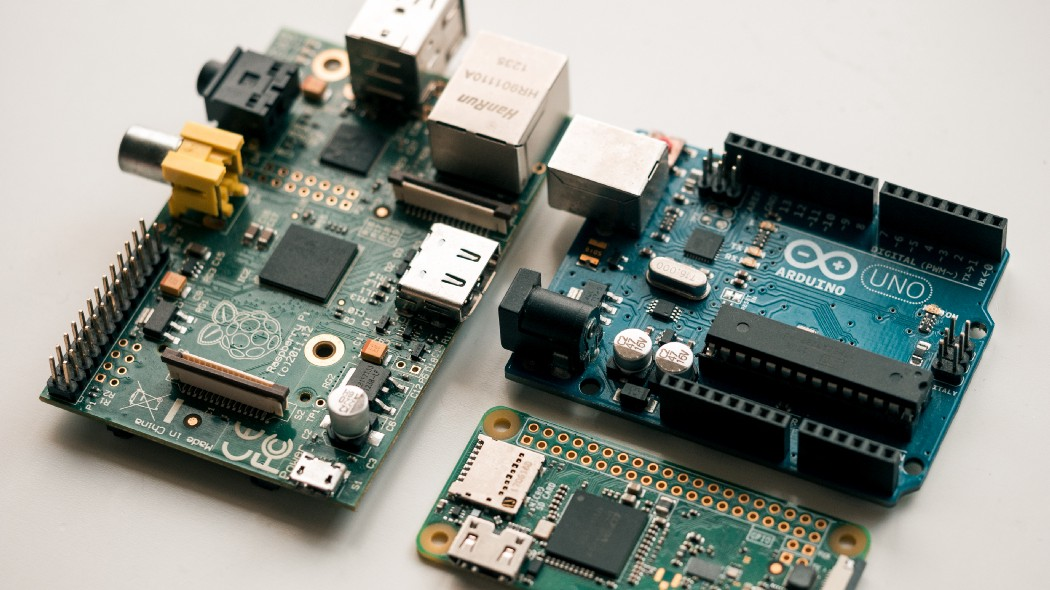
\includegraphics[scale=0.25]{../../figs/hardware_devices.jpg}
    \caption{Quelques cartes pour réseaux intélligents.\label{fig:carte}}
\end{figure}